\documentclass[10pt,a4paper]{article} % tamaño de letra y tipo de papel
\usepackage[utf8]{inputenc}
\usepackage[spanish]{babel} % paquete para que reconozca ñ y tildes
\usepackage{amsmath}
\usepackage{upgreek} 
\usepackage{amsfonts}
\usepackage{amssymb}
\usepackage{graphicx} % paquete para incluir imagenes
\usepackage[margin=1in,bottom=1in]{geometry}
\usepackage{hyperref} % paquete para tener marcadores en el pdf
\usepackage{tikz}
\usetikzlibrary{babel}
\usepackage[siunitx, RPvoltages]{circuitikz}
\usetikzlibrary{bending,arrows.meta,positioning,calc,positioning}
\usepackage{pgfplots}\pgfplotsset{compat=1.13}

\pgfplotsset{width=12cm,legend style={at={(0.11,0.75)},anchor=south},select coords between index/.style 2 args={
		x filter/.code={
			\ifnum\coordindex<#1\def\pgfmathresult{}\fi
			\ifnum\coordindex>#2\def\pgfmathresult{}\fi
		}
}}
\author{Ulloa Daniel}
\begin{document}

\begin{titlepage}
	\hbox{
		\hspace*{0.15\textwidth} % Espacio desde el margen izquierdo
		\rule{1pt}{\textheight} % Linea decorativa
		\hspace*{0.05\textwidth} % Espacio entre la linea y el texto
		\parbox[b]{0.75\textwidth}{ % Caja que restringe el espacio que puede ocupar el texto
			{\noindent\Huge\bfseries Informe de Laboratorio } % Titulo
			\\ 
			[2\baselineskip] 
			{\large \textbf{Tema:} Oscilador con Resistencia Negativa} % Tema
			\\[4\baselineskip]
            {\large \textbf{Cátedra:} Teoría de Circuitos \textsc{II}} % Catedra
            \\[1\baselineskip]
            {\large \textbf{Año:} 2019} % Año
			\\[1\baselineskip]
            {\large \textit{\textbf{Docentes:} % Docentes
                \textnormal{Ing. Costa}, Nicolás. 
                \textnormal{Aux. Consiglio}, Dante}
            }
			\\[1\baselineskip]
            {\large \textit{\textbf{Alumnos:} % Alumnos
                \textnormal{Rodriguez}, Ana Victoria. 
                \textnormal{Ulloa}, Daniel Alejandro}
            }
            \\[6\baselineskip]
            {\large \textbf{Fecha de Entrega:} 11/09/2019}
			\par %Para que el logo aparezca al pie
			\vspace{0.35\textheight} % Ubicacion de la caja desde el margen superior
            \center{
\includegraphics[width=250px]{logo2.png}}
            \\[1\baselineskip]
	}}
\end{titlepage}
\tableofcontents
\newpage
\section{Introducción}
\begin{center}
    \begin{circuitikz}[american voltages,american inductors]
        \draw (0,0) node [op amp](amp){};
        \draw (amp.-) to [C,l=$C$,v_<=$V_{C(0)}$] ++(-2,0) to [L,l=$L$,i>_=$i$] ++(-2,0) to [R,l=$R_1$] ++(-2,0) node[ground]{};
        \draw (amp.-) to[short,*-] ++(0,1.5) coordinate (leftR2) to[R,l=$R_2$] (leftR2 -| amp.out) to[short,-*] (amp.out);
        \draw (amp.out) to [R,l=$R_a$]++(0,-2) coordinate (rightRa);
        \draw (amp.+) to [short]++(0,-1.51) to [short,-*](rightRa) node [right] {$V_p$};
        \draw (rightRa) to [R,l=$R_b$]++(0,-2) node[ground]{};
        \draw (amp.out) to [short,*-o]++(1,0)node [right] {$V_{o(t)}$};	
        \draw (amp.up) --++(0,0.1) node[vcc]{12\,\textnormal{V}};
        \draw (amp.down) --++(0,-0.1) node[vee]{-12\,\textnormal{V}};
    \end{circuitikz} 
\end{center}


El sistema de la figura lleva el nombre de oscilador con resistencia negativa, por inspección, se puede observar que el circuito es una configuración RLC serie acompañada de un Conversor de Impedancias Negativas:
%conversor imp negativa
\begin{center}
    \begin{circuitikz}[american voltages]
        \draw (0,0) node [op amp](amp){};
        \draw (amp.-) to [short,o-*,f<^=$I_1$]++(-2,0) node [left] {$V_1$};
        \draw (amp.-) to[short,*-] ++(0,1.5) coordinate (leftR2) to[generic,l=$Z$] (leftR2 -| amp.out) to[short,-*] (amp.out);
        \draw (amp.out) to [R,l=$R_2$]++(0,-2) coordinate (rightRa);
        \draw (amp.+) to [short]++(0,-1.51) to [short,-*](rightRa);
        \draw (rightRa) to [R,l=$R_1$]++(0,-2) node[ground]{};
        \draw (amp.out) to [short,*-o]++(1,0)node [right] {$V_2$};
    \end{circuitikz}
\end{center}

La impedancia de entrada de este circuito es $Z_{in}=V_1/I_1$. Si las resistencias $R_1$ y $R_2$ son iguales 
 entonces la impedancia $Z_{in}=-Z$. Por lo tanto se puede representar el circuito de la siguiente manera:

\begin{center}
    \begin{circuitikz}[american voltages,american inductors]
        \draw (0,0) -- (0,-1) node[ground]{}; 
        \draw (0,0) to[R, l=$R_1$] (2,0);
        \draw (2,0) to [L,l=$L_1$,i_<=$i_L$] (4,0);
        \draw (4,0) to [C,l=$C_1$,v_>=$V_{C(0)}$] (6,0);	
        \draw (6,0) to [generic, l=$Z_{in}$] (8,0);
        \draw (8,0) -- (8,-1) node[ground]{};
    \end{circuitikz}
\end{center}
Esta impedancia negativa $Z_{in}$ compensa las pérdidas de energía en la resistencia $R_1$ y como consecuencia el circuito se comporta como un oscilador.

El circuito RLC junto al conversor de impedancia negativas conforman un sistema de segundo orden. El modelo teórico de la función de transferencia se muestra a continuación:
\begin{equation}
    H(s)=\dfrac{Y(s)}{U(s)}=\dfrac{K}{s^{2}\tau^{2}+2\xi \tau s+1}
    \end{equation}
    En los sistemas de segundo orden existen tres parámetros a considerar:
    \begin{itemize} 
    	\item k: ganancia estática
    	\item $\xi$: factor de amortiguamiento
    	\item $1/\tau$: frecuencia natural no amortiguada
    \end{itemize}
       La posición de los polos está determinada por el factor de amortiguamiento, $\xi$. 
         \begin{equation}
       p_{1,2}=\frac{1}{\tau}\left(-\xi\pm\sqrt{\xi^2-1}\right)
       \end{equation}
       Para obtener la característica de un oscilador los polos deben ser imaginarios puros, por lo tanto 
       $\xi$ debe ser nula. 
  

    %\xi=0$

\section{Objetivos}
\begin{itemize}
    \item Modelar e interpretar el Circuito
    \item Obtener la respuesta temporal de la tensión de salida y graficarla en Mathematica
    \item Realizar un barrido paramétrico sobre la resistencia $R_B$ y observar las diferentes respuestas.
\end{itemize}

\section{Modelado Matemático}
Para modelar el circuito se tuvieron en cuenta algunas consideraciones
%\begin{center}
%    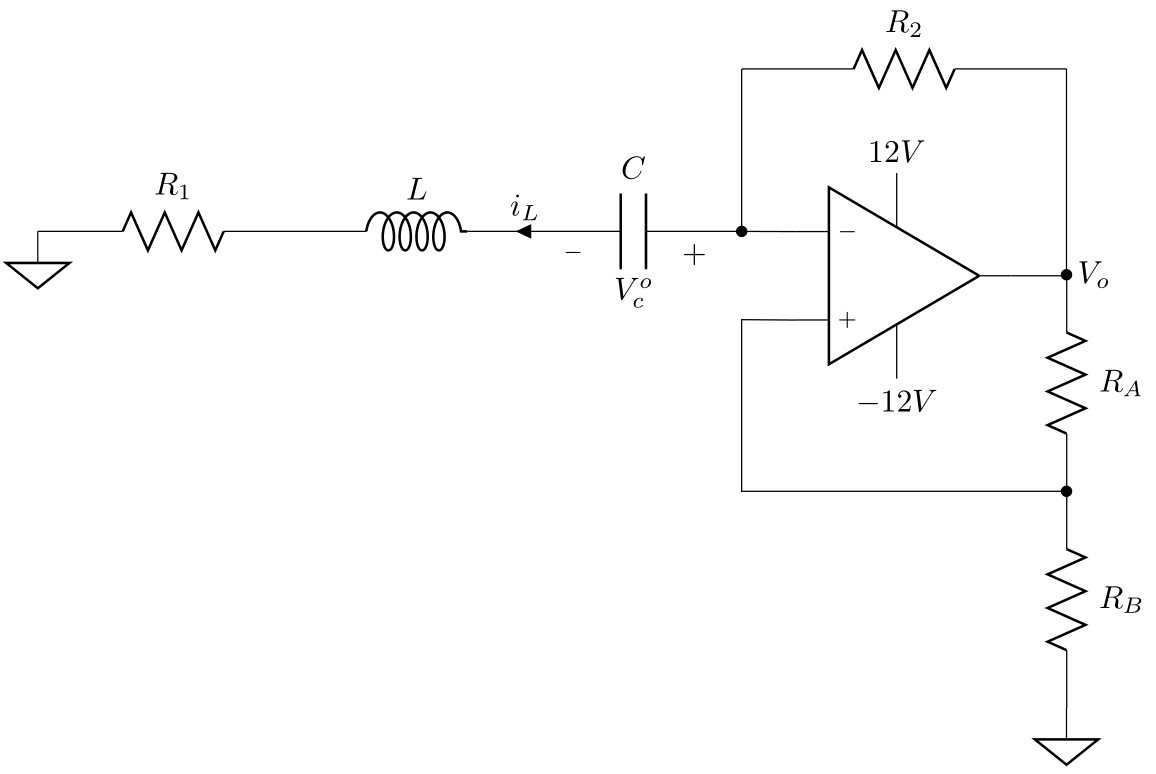
\includegraphics[width=300px]{circuito}
%\end{center}

\begin{itemize}
    \item El amplificador operacional es ideal
    \item La tensión inicial en el capacitor es $V_{C(0)}$
    \item La corriente del capacitor se expresará de forma diferencial
    %\item La corriente en el inductor es la misma que en el capacitor y en las resistencias $R_1$ y $R_2$
    \item La entrada del sistema es la tensión inicial del capacitor
    \item La salida del sistema es la tensión a la salida del Amplificador Operacional
\end{itemize}

\begin{circuitikz}[american voltages,american inductors]
	\draw (0,0) node [op amp](amp){};
	\draw (amp.-) to [C,l=$C$,v_<=$V_{C(0)}$] ++(-2,0) to [smeter, t=A, l=$i\text{=}C\frac{dV}{dt}$]++(-2,0) to [L,l=$L$,i>_=$i$] ++(-2,0) to [R,l=$R_1$] ++(-2,0) node[ground]{};
	\draw (amp.-) to[short,*-] ++(0,1.5) coordinate (leftR2) to[R,l=$R_2$,i<=$i$] (leftR2 -| amp.out) to[short,-*] (amp.out);
	\draw (amp.out) to [R,l=$R_a$]++(0,-2) coordinate (rightRa);
	\draw (amp.+) to [short]++(0,-1.51) to [short,-*](rightRa) node [right] {$V_p$};
	\draw (rightRa) to [R,l=$R_b$]++(0,-2) node[ground]{};
	\draw (amp.out) to [short,*-o]++(1,0)node [right] {$V_{o(t)}$};	
	\draw (amp.up) --++(0,0.1) node[vcc]{12\,\textnormal{V}};
	\draw (amp.down) --++(0,-0.1) node[vee]{-12\,\textnormal{V}};	
\end{circuitikz}
Para la primera ecuación se analizó el nodo $V_n$, en donde se tiene que:
\begin{equation}   
i(t)=i_{R2}(t)
\end{equation}
Expresando las corrientes en términos forma diferencial
\begin{equation}
i(t)=C*V_{c}'(t)
\end{equation} 
\begin{equation}
i_{R2}(t)=\frac{V_{o}(t)-V_{n}(t)}{R_{2}}
\end{equation}

\begin{equation}
V_{p}(t)=\frac{R_{b}* V_{o}(t)}{R_{a}+R_{b}}
\end{equation}
Donde las tensiones $V_{n}(t)$ y $V_{p}(t)$ son iguales al considerar que el amplificador operacional es ideal.


De esta manera se obtiene la primera ecuación de nuestro sistema, a la cual se le aplicó la transformada de Laplace. 
\begin{equation}
eq1:C* (s V_{c}(s)-V_{c}(t))-\frac{R_{a}* V_{o}(s)}{R_{2} R_{a} +R_{2} R_{b}}
\end{equation}
Para la segunda ecuación se analizó la malla que contiene a los componentes $R_{1},R_{2}, C$ , $L$ y $V_{o}(s)$ 
\begin{equation}
\ V_{o}(t)=\ V_{c}(t)+ V_{l}(t)+ V_{r}(t)
\end{equation}
\begin{equation}
V_{o}(t)=C*L*V_{c}''(t)+ C*(R_{1}+R_{2})*V_{o}'(t)+V_{c}(t)
\end{equation}
Nuevamente se aplico la transformada de Laplace, obtiendo la segunda ecuación
\begin{equation}
eq2 = V_{c}(s) - V_{o}(s) + C(R_{1} + R_{2})(s*V_{c}(t) - v_{0}(t)) + 
LC(s^{2}*V_{c}(t) - s*v_{0}(t))
\end{equation}
Con estas dos ecuaciones es posible obtener las tensiones de salida y entrada del sistema y su función de transferencia 
\begin{equation}
H(s)=\frac{C R_{2} (R_{a}+R_{b})}{s*R_{a}C (s*\text{L} +R_{1}+2 R_{2})-s*\text{C}R_{2} R_{b} -R_{a}}
\end{equation}
Reordenando la función de transferencia
\begin{equation}
H(s)=\frac{\frac{CR_{2}*(R_{a}+R_{b})}{R_{a}}}{-1+(-CR_{1}+\frac{CR_{2}R_{b}}{R_{a}})s-(LC)s^{2}}
\end{equation}
\\
Comparando la función de transferencia obtenida con la función del modelo teórico se determinaron los parámetros $\xi$, $\tau$ y k 
\begin{equation}
K=\frac{CR_{2}*(R_{a}+R_{b})}{R_{a}}
\end{equation}
\begin{equation}
\tau=\sqrt{LC}
\end{equation}
\begin{equation}
\xi=\dfrac{-CR_{1}+\frac{CR_{2}R_{b}}{R_{a}}}{2\sqrt{LC}}
\end{equation}

Un coeficiente de amortiguamiento nulo implica que las resistencias $R_1$,$R_2$,$R_a$ y $R_b$ deben ser iguales. 


\section{Respuesta Temporal}
Para la respuesta temporal del oscilador aplicamos la antitransformada o inversa de Laplace obteniendo la respuesta al escalón
\begin{equation}
    V_{o(t)}=\frac{d}{\sqrt{b}}\left[e^{\left(-a-\dfrac{\sqrt{b}}{c}\right)t}-e^{\left(-a+\dfrac{\sqrt{b}}{c}\right)t}\right]
\end{equation}

En donde: 
\begin{equation}
a=\frac{R_{1}}{2 \text{L}}+\frac{R_{2} R_{b}}{2 \text{L} R_{a}}+\frac{R_{2}}{\text{L}}
\end{equation}
\begin{equation}
b=(\text{C} R_{1} R_{a} +2 \text{C} R_{2} R_{a} +\text{C} R_{2} R_{b})^2-4 \text{C} \text{L} R_{a}^2
\end{equation}
\begin{equation}
c=2 \text{L} \text{C} R_{a}
\end{equation}
\begin{equation}
d= (R_{a}+R_{b})R_{2}C
\end{equation}

Se propuso valores para los elementos del sistema y se gráfico la respuesta temporal, obteniendo el siguiente gráfico
%mathamticaaaaa

\begin{equation}
R=1000
\end{equation}
\begin{equation}
L=10mH
\end{equation}
\begin{equation}
C=1u F
\end{equation}
\section{Barrido Paramétrico}
Para observar el comportamiento del circuito ante cambios en el valor de la resistencia equivalente se realiza un barrido paramétrico en LTSpice:
\begin{center}
    \begin{circuitikz}[american voltages, american inductors]
	\draw (0,0) node [op amp](amp){};
	\draw (amp.-) to [C=1<\micro\farad>] ++(-2,0) to [L=10<\milli\henry>] ++(-2,0) to [R=1<\kilo\ohm>] ++(-2,0) node[ground]{};
	\draw (amp.-) to[short,*-] ++(0,1.5) coordinate (leftR2) to[R=1<\kilo\ohm>] (leftR2 -| amp.out) to[short,-*] (amp.out);
	\draw (amp.out) to [R=1<\kilo\ohm>]++(0,-2) coordinate (rightRa);
	\draw (amp.+) to [short]++(0,-1.51) to [short,-*](rightRa);
	\draw (rightRa) to [R,l=$\{Rb\}$]++(0,-2) node[ground]{};
	\draw (amp.out) to [short,*-o]++(1,0)node [right] {$V_{o(t)}$};
	\node at (-5.6,-2.5){.tran 20ms uic};
	\node at (-4,-3){.step param Rb list 0.99k 1k 1.2k};	
	\draw (amp.up) --++(0,0.1) node[vcc]{12\,\textnormal{V}};
	\draw (amp.down) --++(0,-0.1) node[vee]{-12\,\textnormal{V}};
\end{circuitikz}
\end{center}

Se obtuvieron las siguientes respuestas

\begin{center}
    \begin{tikzpicture}[
        ]
        \begin{axis}[
        xlabel=$Tiempo$, ylabel=$V_{o(t)}$, grid=major,legend entries={$850\Omega$,$990\Omega$,$1000\Omega$,$1005\Omega$}
        ]
        \addplot[color=green,
        select coords between index={1}{400},
        filter discard warning=false, unbounded coords=discard
        ] table [x index=0, y index=1]{r850.txt};
        \addplot[color=blue,
        select coords between index={1}{400},
        filter discard warning=false, unbounded coords=discard
        ] table [x index=0, y index=1]{r990.txt};
        \addplot[color=red,
        select coords between index={1}{400},
        filter discard warning=false, unbounded coords=discard
        ] table [x index=0, y index=1]{r1k.txt};
        \addplot[color=black,
        select coords between index={1}{400},
        filter discard warning=false, unbounded coords=discard
        ] table [x index=0, y index=1]{r1005.txt};
    \end{axis}
    \end{tikzpicture}
\end{center}

\section{Conclusión}
\end{document} 
















